% !Mode:: "TeX:UTF-8"
\chapter{项目所用数据的搜集与处理}
本章的内容是为了构造程序所需要的数据结构,实现根据参数来爬取指定经纬度的osm地图数据,然后转化为shp地图数据,读取shp地图数据来构造图的数据结构---邻接矩阵。
\section{数据爬取}
\subsection{爬取osm数据}
OPen Street Map简称OSM,是一个由网络大众共同打造的免费开源服务,在上面你可以下载指定经纬度的地图信息,
该组织由史蒂夫·克斯特与2004年7月创立,2006年4月OSM基金会成立,他鼓励社区的用户自由的发布地理数据,并与社区所有人分享并使用地理数据,
为了搜集本项目的数据,我们在osm中采用爬虫技术爬取osm文件。下面是分析过程:\\
\begin{figure}[H]
    \centering
    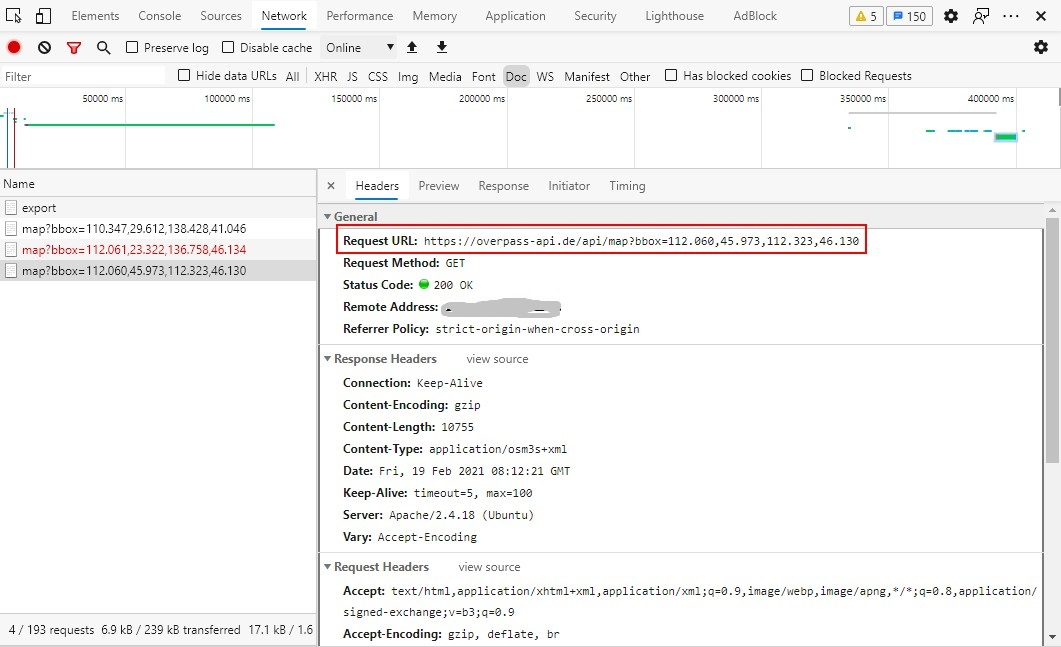
\includegraphics[width=13cm]{figure/osm_1.jpg}
    \caption{调试信息General项}
    \label{fig-tsxx1}
\end{figure}
我们从上图可以看出下载的osm文件的请求地址,其中请求类型为GET表明该数据的请求信息加载在网址中,且成功返回数据,状态码为200,返回的数据大小为10755。然后我们查看该请求的请求头信息:\\
\begin{figure}[H]
    \centering
    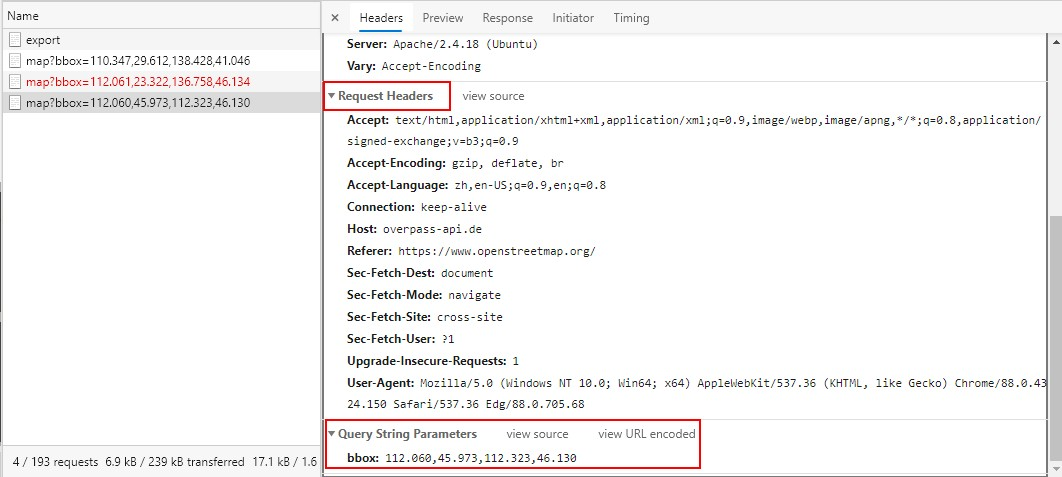
\includegraphics[width=13cm]{figure/osm_2.jpg}
    \caption{调试信息请求头}
    \label{fig-tsxx2}
\end{figure}
根据请求头我们发现该网站在请求头中并不存在验证本机的信息,\\
说明该网址并不存在反爬虫,所需无需手动构造请求头,让程序请求时自动生\\
成即可,所以程序为:
\newline
\begin{lstlisting}[
    language={Python},
    caption={爬取osm数据代码},
    label={download-osm},]
import requests
import json
import sys
import zipfile
for arg in sys.argv:
    bbox = arg # 经纬度信息作为参数传递
osm_path = '/TSP_hopfield/shp_distance/map'
zip_file = '/TSP_hopfield/shp_distance/map.zip'
def download_osm():
    url = 'https://overpass-api.de/api/map?bbox='+ bbox # 115.3141,38.8425,115.4748,38.9303
    myfile = session.get(url , allow_redirects=True)
    open ( osm_path, 'wb').write(myfile.content)
session = requests.session()
# 下载osm文件
download_osm()
\end{lstlisting}
为了使得其余程序能够直接调用此文件来下载特定区域内的osm数据,我们的程序会读取命令行列表,来动态下载地图数据,下面为了将地图数据转变为计算机好读取的格式我们将其转化为shp类型地图文件。
\subsection{转化成shp数据}
首先打开 "https://geoconverter.hsr.ch/" 网站,如下所示:\\
\begin{figure}[H]
    \centering
    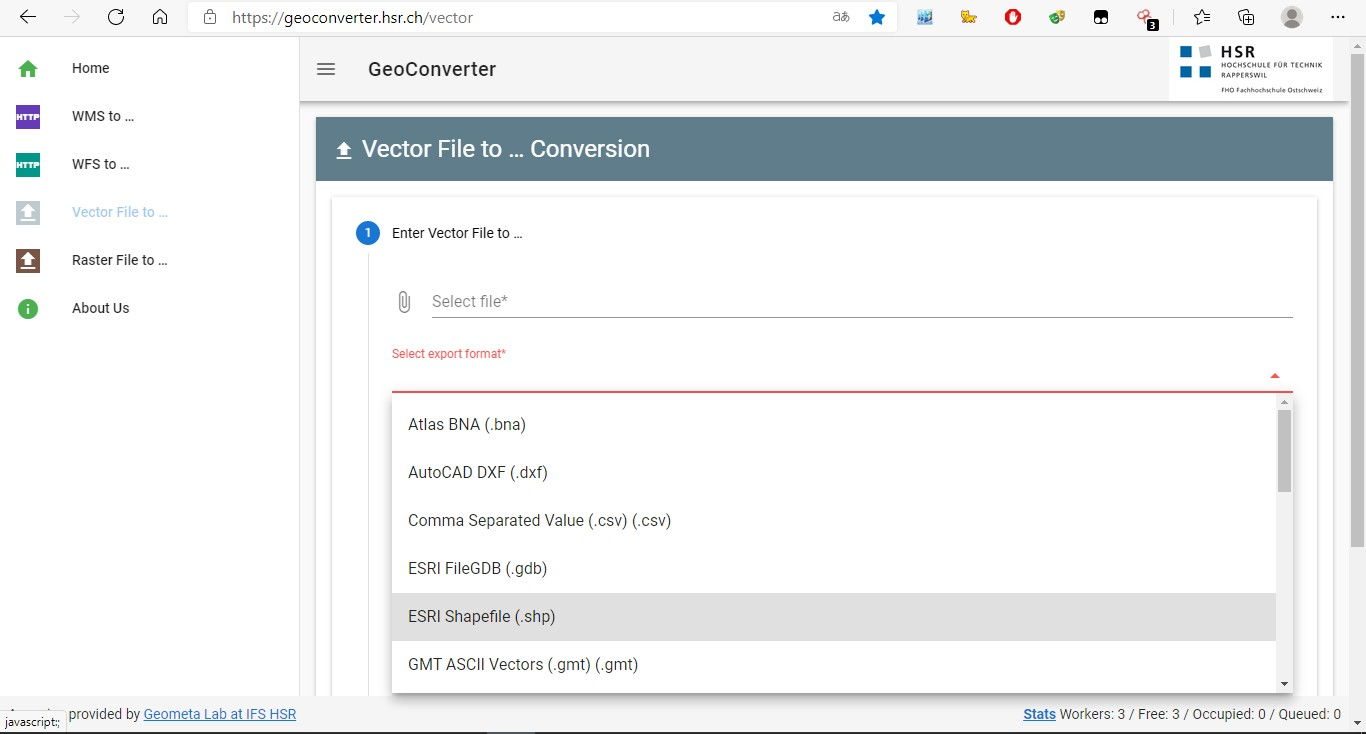
\includegraphics[width=13cm]{figure/shp_1.jpg}
    \caption{进入geoconverter网站}
    \label{fig-geo}
\end{figure}
我们上传osm文件,并调整转化格式。然后点击转换,即可下载转换后的文件,但是为了能够自动化的进行文件转换,我们采用爬虫技术,来实现文件的上传,转换,下载的步骤,为了模拟该流程,我们首先进行一次数据的提交转换,来观察其过程。\\
\begin{figure}[H]
    \centering
    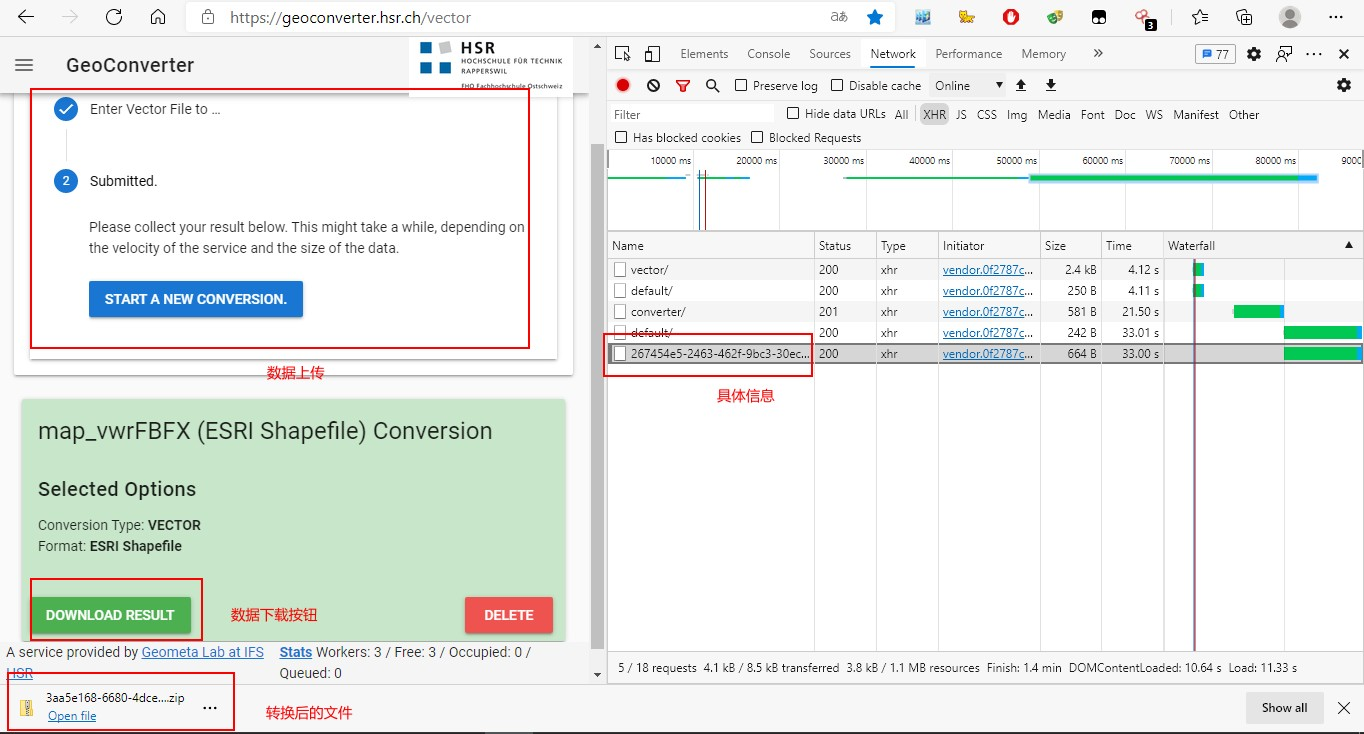
\includegraphics[width=13cm]{figure/shp_2.jpg}
    \caption{模拟提交转换文件}
    \label{fig-mntj}%模拟提交
\end{figure}
其中转化后的shp的文件在下载的zip压缩文件内,他被分为了3个部分分别为,路网,水网,建筑网三个文件,我们程序只需提取路网文件即可。
再上图中我们在调试XHR栏目中可以看到许多请求过程文件,但是值得注意的只有converter/请求与由长数字字母构成的267454e5-2463-462f-9bc3-30ecbe41956d/请求,
并且查看文件发送时间后发现,converter/请求发送时间较早,而267454e5-2463-462f-9bc3-30ecbe41956d/请求发送较晚,
并且在查看请求内容后我们发现,converter/请求时发送文件的并返回267454e5-2463-462f-9bc3-30ecbe41956d/请求名称即:\\
\begin{figure}[H]
    \centering
    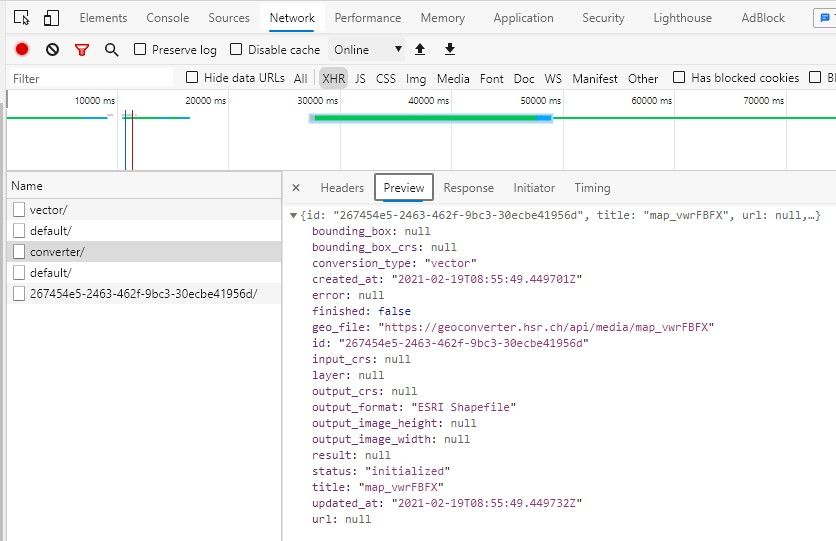
\includegraphics[width=13cm]{figure/shp_3.jpg}
    \caption{请求文件信息}
    \label{fig-qqwjxx}%请求文件信息
\end{figure}
所以我们的程序会对multipart/form-data请求进行模拟,通过post请求将文件发送到服务器。并保存服务器响应数据,读取响应数据的id值,并以此构造第二次请求的url,这就是图中的267454e5-2463-462f-9bc3-30ecbe41956d/请求,请求详细信息如下:\\
\begin{figure}[H]
    \centering
    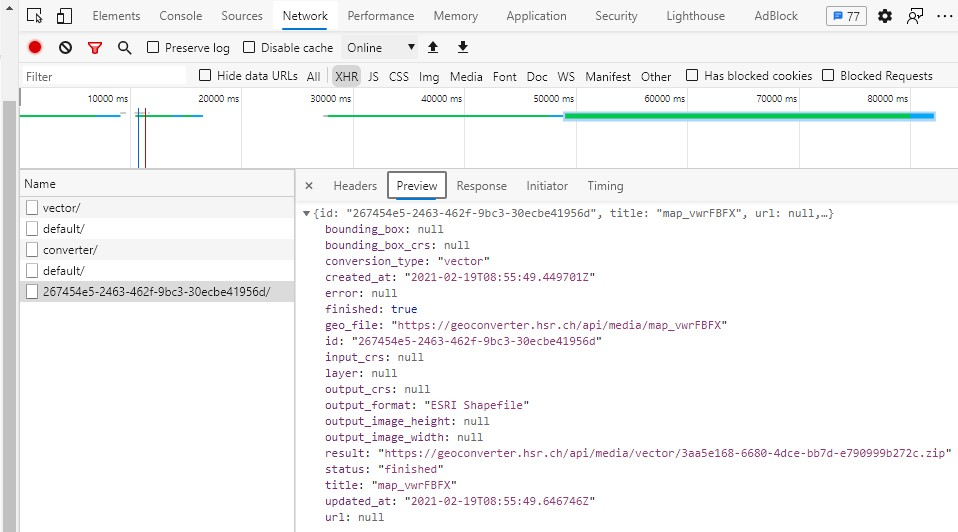
\includegraphics[width=13cm]{figure/shp_4.jpg}
    \caption{第二次请求信息}
    \label{fig-drcqqxx}%第二次请求信息
\end{figure}
从以上的信息中提取到转化后的文件下载地址。在此次模拟提交中是:"https:\\
//geoconverter.hsr.ch/api/media/vector/3aa5e168-6680-
4dce-bb7d-e790999b272c.zip",转换结束,然后我们以此来编写代码来代替人工进行自动化请求转化下载步骤,然后解压文件提取shp文件,代码如下:\\
\begin{lstlisting}[
        language = {Python},
        caption = {转化为shp数据},
        label = {download-shp},
]
    second_headers = {
    'authority': 'geoconverter.hsr.ch',
    'method': 'GET',
    'path': '',
    'scheme': 'https',
    'accept': 'application/json, text/plain, */*',
    'accept-encoding': 'gzip, deflate, br',
    'accept-language': 'zh,en-US;q=0.9,en;q=0.8',
    'referer': 'https://geoconverter.hsr.ch/vector',
    'sec-fetch-dest': 'empty',
    'sec-fetch-mode': 'cors',
    'sec-fetch-site': 'same-origin',
    'user-agent': 'Mozilla/5.0 (Windows NT 10.0; Win64; x64) AppleWebKit/537.36 (KHTML, like Gecko) Chrome/87.0.4280.88 Safari/537.36 Edg/87.0.664.66',
}
# 将osm文件转化为shp文件

#       构造 multipart/form-data 用来上传osm文件
files = {'geo_file': ('file', open(osm_path, 'rb'),'application/octet-stream'),
         'conversion_type':( None, 'vector'),
         'output_format':( None, 'ESRI Shapefile')
         }
#       不断的请求上传直到响应状态码正确
while True:
    res = session.post(url, files=files)
    if res.status_code // 100 == 2:
        break
#       获取响应id
id = res.text.split('"')[3]
#       构造请求头,准备进行第二次请求,下载转换的zip文件
second_url = 'https://geoconverter.hsr.ch/api/converter/' + id + '/'
path = '/api/converter/'+ id +'/'
second_headers['path'] = path
#       不断的进行第二次请求直到返回正确的zip文件下载地址
while True:
    res = session.get(second_url, headers = second_headers)
    if res.status_code // 100 == 2 and json.loads(res.text)['result'] != None:
        break
#       将zip下载地址从 text-->json 中提取出来
res_dict = json.loads(res.text)
shp_download_url = res_dict['result']
# 压缩文件名称
yasuo_file = shp_download_url.split("/")[-1].split('.')[0]
# 下载shp的压缩文件并保存
myfile = session.get(shp_download_url , allow_redirects=True)
open ( zip_file, 'wb').write(myfile.content)
with zipfile.ZipFile(zip_file) as zf:
    zf.extractall()
shp_path = '/TSP_hopfield/shp_distance/' + yasuo_file + '/converted.shp'
print(shp_path)
\end{lstlisting}
\section{图数据结构的构建}
\subsection{读取line数据}
在matlab中读取shp文件数据,我们可以得到$n \times 1 \quad struct$的数据其中$n$表示线的组数,其line数据包含以下数据:
% Table generated by Excel2LaTeX from sheet 'Sheet1'
\begin{table}[htbp]
    \centering
    \caption{line字段}
      \begin{tabular}{|l|r|l|}
      \hline
      字段    & 含义 \\
      \hline
      Geometry & 拓扑结构 \\
      BoundingBox & 边界框 \\
      X     & 线段各点的x坐标 \\
      Y     & 线段各点的y坐标 \\
      osm\_id & 路段id \\
      name  & 路段名称 \\
      highway & 道路类别 \\
      waterway & 水路类别 \\
      aerialway & 空中路段类别 \\
      barrier & 障碍物 \\
      man\_made & 人造物 \\
      z\_order & 高度 \\
      other\_tags & 其他标签 \\
      \hline
      \end{tabular}%
    \label{tab:lzd}%line字段
\end{table}% 
下面我们根据以上信息初步生成邻接矩阵,其基本思想为遍历$line$数据结构的每个元素,将每个元素的X,Y项分别输入一个存储已知点集的数组中,我们称其为$x_{pos},y_{pos}$。然后对$line$中的每个元素X,Y相邻的坐标点进行距离计算并存储到邻接矩阵distance中。由于各个路段之间村子啊交点,但line数据结构并不会主动将这些交点标注出来,所以我们准备用快速排斥与跨立算法对线集中的交点进行求解。
\subsection{求交点}
在判断平米拿上两条线段是否相交时,我们采用快速排斥与跨立实验的算法,其基本思想为,首先通过快速排斥实验来对不满足条件的情况进行排除,然后对剩余情况用跨立实验进行具体判断并求解。
\subsubsection{快速排斥}
假设二维平面上存在两个线段,$(P_1,P_2),(Q_1,Q_2)$,以$P_1,P_2$组成的线段为对角线做矩形R,以$Q_1,Q_2$为对角线做矩形T,当两个矩形不相交时两个线段肯定不相交,但两个线段不相交时,两个矩形可能会相交。
\begin{figure}[H]
    \centering
    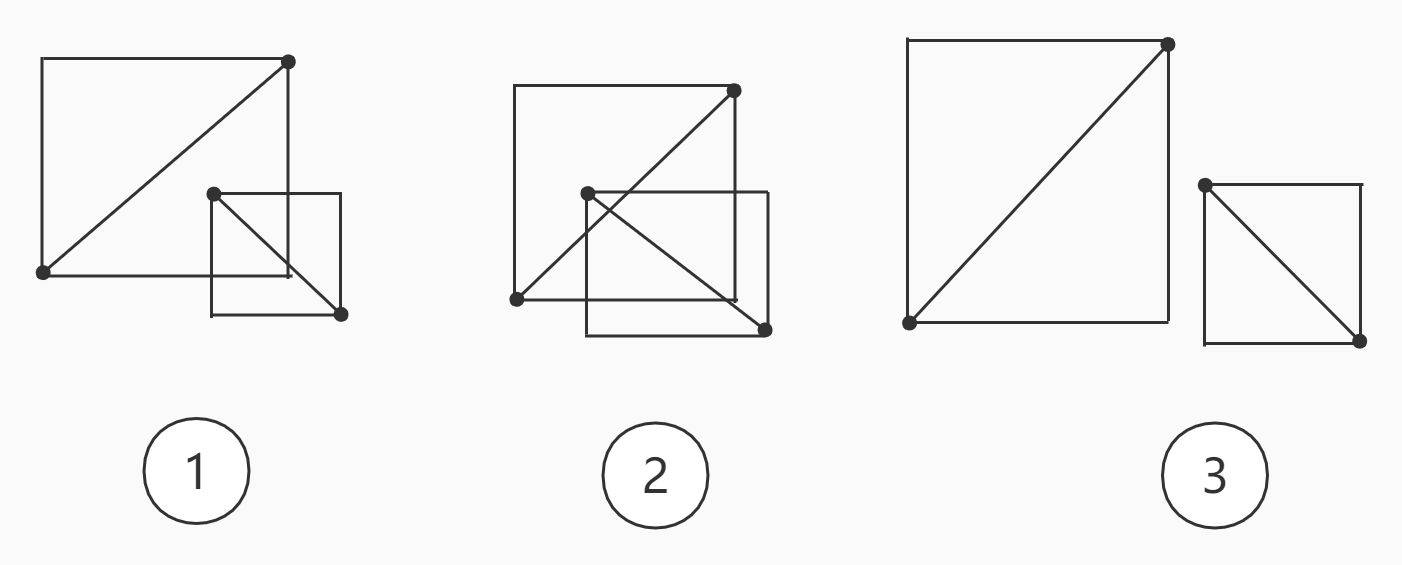
\includegraphics[width=13cm]{figure/jdsy.jpg}%交点实验
    \caption{快速排斥与跨立实验}
    \label{fig:jdsy}
\end{figure}
其中第一种情况通过了快速排斥实验但并未通过跨立实验,第二种情况通过了快速排斥实验,并且也通过了跨立实验,第三种情况并未通过快速排斥实验,直接可以得出结论,不存在交点。\\
在所以在快速排斥中的矩阵相交条件为:
\begin{align}
    min(p_1.x,p_2.x) \le max(q_1.x,q_2.x) \&\& \\
    min(q_1.x,q_2.x) \le max(p_1.x,p_2.x) \&\& \\
    min(p_1.y,p_2.y) \le max(q_1.y,q_2.y) \&\& \\
    min(q_1.y,q_2.y) \le max(p_1.y,p_2.y);
\end{align}
如果通过了快速排斥实验,也不能直接得出结论二者有交点,而是在通过跨立实验得到结果。
\subsubsection{跨立实验}
\begin{figure}[H]
    \centering
    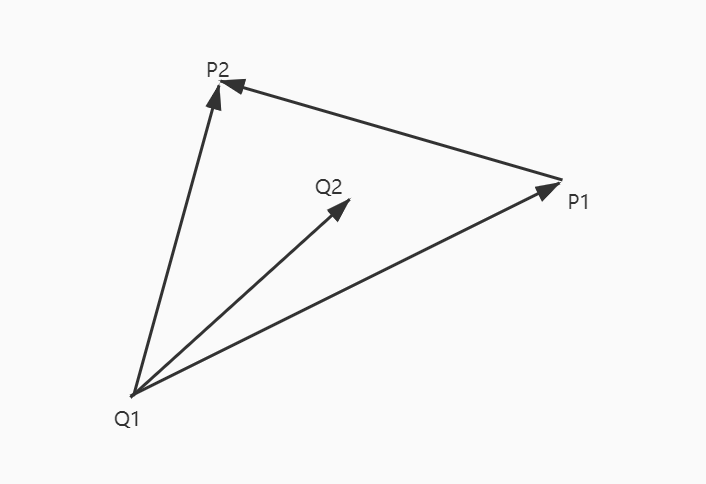
\includegraphics[width=13cm]{figure/kl.jpg}%跨立
    \caption{跨立实验}
    \label{fig:kl}
\end{figure}
若线段$P_1P_2$跨过了线段$Q_1Q_2$,那么$P_1P_2$就在$Q_1Q_2$的两侧,所以将:
\begin{align}
    ((P_1-Q_1) \times (Q_2-Q_1)) *((Q_2-Q_1) \times (P_2-Q_1)) > 0 \label{kl1}
\end{align}
记为条件1,同理$Q_1Q_2$分布在$P_1P_2$两侧的条件为:
\begin{align}
    ((Q_1-P_1)\times(P_2-P_1))*((P_2-P_1)\times(Q_2-P_1))>0 \label{kl2}
\end{align}
记为条件2,满足以上两个条件两线段才会相交。运行程序我的得到运行前后邻接矩阵的点数对比:\\
\begin{table}[H]
    \centering
    \caption{运行前后点数对比}
      \begin{tabular}{|l|r|}
      \hline
      点数对比  & \multicolumn{1}{l|}{点数} \\
      \hline
      求交点前  & 3104 \\
      求交点后  & 4145 \\
      \hline
      \end{tabular}%
    \label{tab:dsdb}%点数对比
  \end{table}%  
可以看出运行前后,在该图中共找到1041个交点,改善了图的连通性,使得路径求解称为可能,下面我们给出求解邻接矩阵算法的完整算法流程图,其中我们设shp文件读取后的数据为$Map$,$Map$的每个元素记为$line$,$line$中的元素构成如(\ref{tab:lzd})所示。
\begin{figure}[H]
    \centering
    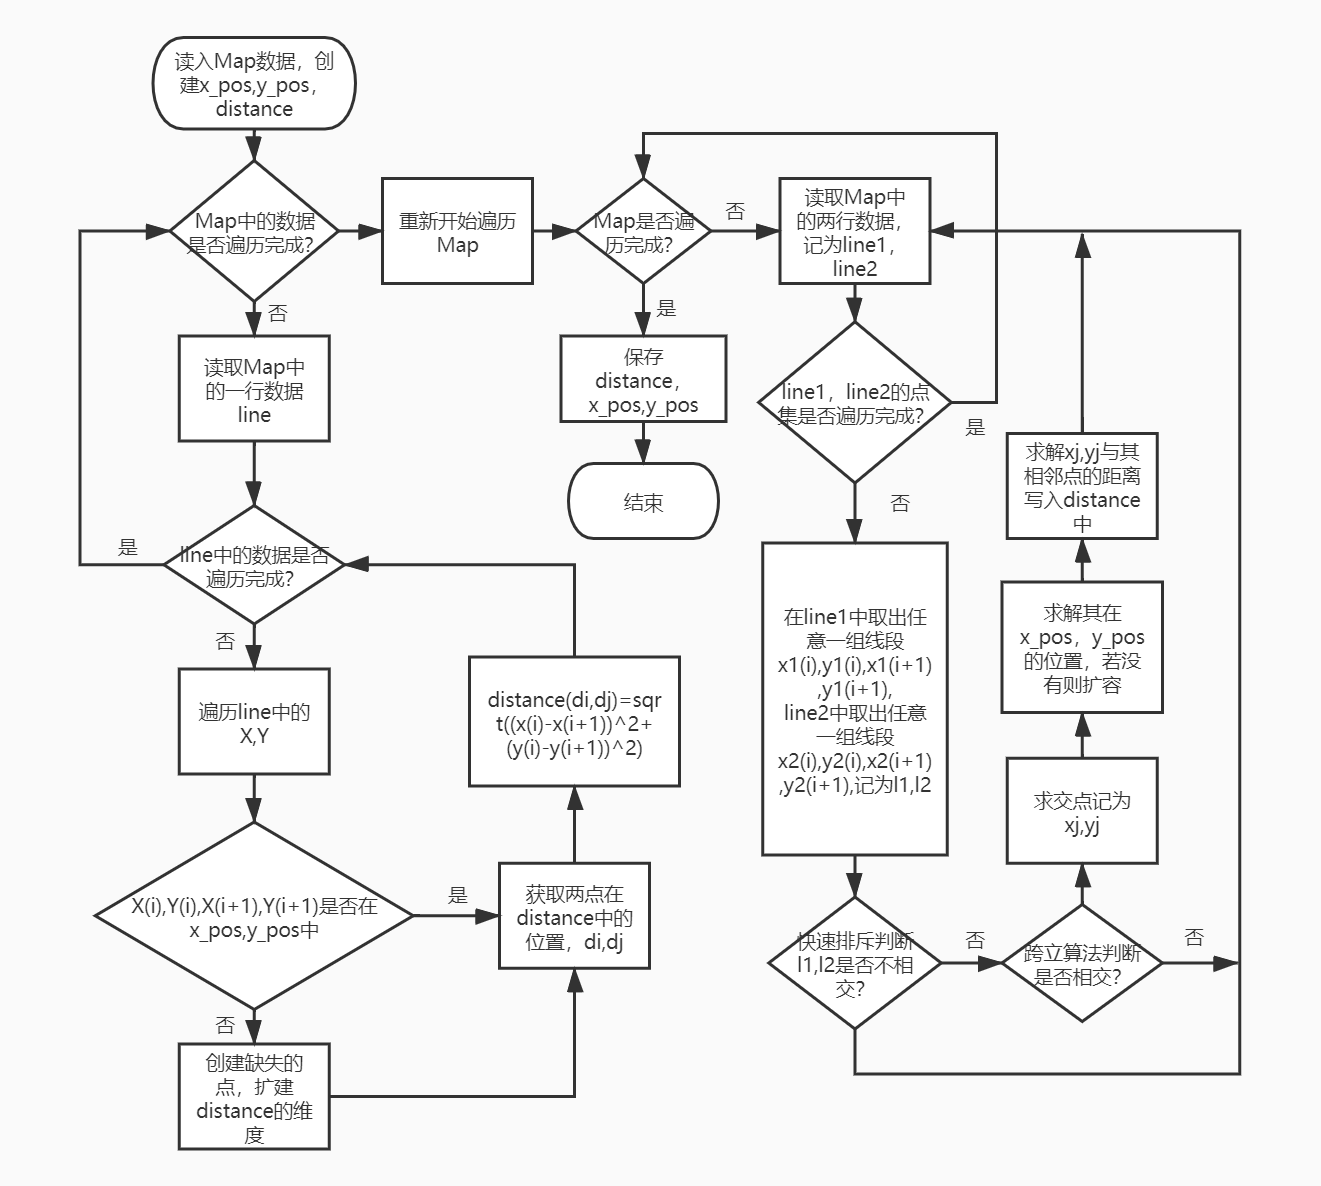
\includegraphics[width=13cm]{figure/create_distance.jpg}%交点实验
    \caption{邻接矩阵构造算法}
    \label{fig:ljjzgzsf}%邻接矩阵构造算法
\end{figure}
以上为数据的所有准备工作,下一章的项目实现将以此数据为依据对路径进行规划。